\documentclass[a4paper,12pt,notitlepage]{article}
\usepackage[utf8]{inputenc}
\usepackage[brazil]{babel}
\usepackage{listings}
\usepackage{graphicx}
\graphicspath{ {imagens/} }
\usepackage{hyperref}

\title{Experimento 1 - Comparação de absorção de detergente em quatro marcas de papel-toalha}
\author{Grupo 1 & 
Alan Oliveira França - 11/0057830 &
Alisson Moreira Ferreira - 11/0106946 &
Augusto Cesar Ribeiro Nunes - 13/0103004 &
Davi Souza Botelho - 12/0029057 & 
Thalyta Brito dos Santos - 12/0023075}
\date{Abril 2016}

\begin{document}
\maketitle
\clearpage

\begin{abstract}
    Este experimento completamente casualizado avaliou a capacidade de absorção de detergente em quatro tipos diferentes de papel-toalha: Snob, Coquetel, Stylus e Maxim. A medida escolhida para investigar a capacidade de absorção foi a diferença entre o peso do papel-toalha após a exposição ao detergente em relação ao peso antes da exposição. O Modelo de Médias escolhido mostrou que há diferença significativa entre as Médias dos Tratamentos, Posteriormente, foram utilizados Contrastes Ortogonais em \ref{sec:co} e Comparação com o Melhor em \ref{sec:cm} para comparação, e concluiu-se que nem sempre o papel-toalha mais caro é o melhor.
\end{abstract}

\section{Introdução}

O papel toalha é um produto multi uso fabricado em celulose e que possui muitas utilidades, como absorção de líquidos, retenção da umidade, secagem das mãos e limpeza em geral. Os papeis toalha são descartáveis resultando em não acúmulo de germes. Além do mais, o papel toalha é um item básico em uma cozinha e devido ao seu poder absorvente, pode ser utilidade para inúmeras finalidades. 
O objetivo deste estudo é realizar um experimento completamente casualizado e com um fator para testar a capacidade de absorção de quatro tipos de marcas de papel toalha. No presente experimento, o líquido utilizado foi o detergente de cozinha. A análise será fundamentada em comparações para mostrar as possíveis diferenças entre as marcas para a absorção do detergente. Outra questão será levantada, a existência da relação entre o preço e a capacidade de absorção, ou seja, marcas mais caras tendem a absorver mais o líquido do que as baratas? Para discorrer sobre essas questões serão aplicadas técnicas de delineamento experimental e análise do custo benefício.

\section{Materiais}

\begin{itemize}
    \item 1 pacote de papel-toalha da marca Snob, produto Multiuso Max Embalagem Econômica, contendo 2 rolos de papel toalha folha dupla, cada um com 120 toalhas de 19cm x 22cm. O papel-toalha desta marca é referido como \textbf{Tratamento 1};
    \item 1 pacote de papel-toalha da marca Coquetel, produto Multiuso, contendo 2 rolos de papel-toalha folha dupla, cada um com 60 toalhas de 19cm x 21,5cm. O papel-toalha desta marca é referido como \textbf{Tratamento 2};
    \item 1 pacote de papel-toalha da marca Stylus, produto Multiuso , contendo 2 rolos de papel-toalha folha dupla, cada um com 50 toalhas de 22cm x 20cm cada. . O papel-toalha desta marca é referido como \textbf{Tratamento 4};
    \item 1 pacote de papel-toalha da marca Maxim, produto taltaltaltal, contendo 2 rolos de papel-toalha folha dupla, cada um com 60 toalhas de 22 x 20 cada. O papel-toalha desta marca é referido como \textbf{Tratamento 3};
    \item 1 forma de alumínio de 12cm x 27cm;
    \item 1 frasco de 500 mL detergente da marca Ypê, produto neutro;
    \item 20 copos plásticos de marca genérica, de capacidade 300 mL;
    \item 1 pinça metálica genérica;
    \item 1 balança de mesa de precisão de um centigrama (0,01 g). A alta precisão da balança mostrou-se um dificultador das medições, já que o peso do conjunto copo e papel aumentava gradativamente. Esse efeito inesperado pode ser atribuído a uma miríade de fatores: o dispositivo estaria descalibrado, a presença de computadores e celulares próximos à mesa de trabalho poderiam estar causando interferência eletromagnética na balança, uma flutuação na corrente elétrica poderia estar causando uma falha de compensação nos leitores da balança etc., então resolveu-se por arredondar as medições na ordem dos decigramas (0,1 g) em nome da simplicidade experimental. Entendeu-se que o ganho em ordem de grandeza de medição seria marginal, e não compensaria a introdução de uma imprecisão arbitrária na variável resposta;
    \end{itemize}
    
    O Anexo B (\ref{anexo:B}) contém fotos dos procedimentos adotados.

\section{Procedimentos}\label{sec:procedimentos}
\begin{enumerate}
    \item Para cada marca de papel, foram destacadas todas as folhas de um dos rolos e utilizando um gerador de números aleatórios (ver o Anexo A (\ref{anexo:A})) de maneira a selecionar aleatoriamente 5 folhas de papel-toalha em cada Tratamento; 
    \item Para controlar a variação das diferentes dimensões das folhas de cada marca, foi realizado um procedimento de uniformização das observações que consistiu em recortá-las em quadrados de 10cm x 10cm - 100$cm^2$ ou 0,01$m^2$ de área;
    \item Cada folha de papel foi colocada dentro de um copo descartável e pesada em uma balança, esta medida foi anotada como o \textbf{peso seco} do papel; \footnote{Note que, a rigor, este \textbf{peso seco} refere-se ao conjunto copo+papel. Essa distinção não é estritamente necessária pois a medida de interesse é a diferença entre o peso após a absorção e o \textbf{peso seco}, e o mesmo copo plástico é utilizado nos dois dois estágios do processo} 
    \item Os papeis foram colocados em uma forma contendo 500 mL de detergente, depositados de modo que repousassem sobre a camada de detergente, e evitando que tocassem a borda da mesma;
    \item O repouso do papel sobre o detergente teve duração de 180 segundos (3 minutos). Para cada folha, foi observado se houve ou não \textbf{saturação} da mesma, i.é., se a folha em algum instante desses 180 segundos ficou completamente umedecida pelo detergente. Esta variável é denominada \textbf{tempo de saturação};
    \item Passados os 180 segundos da imersão no detergente, o papel foi retirado da forma utilizando-se uma pinça comum, e durante 60 segundos (1 minuto) foi deixado que o excesso de detergente escorresse pela folha. 
    \item Passados os 60 segundos de escorrimento, o papel foi recolocado no copo plástico e novamente pesado. Esta medida é o \textbf{peso úmido} do papel\footnote{Novamente, aqui o peso efetivamente medido é o do conjunto copo plástico + folha de papel toalha após os 180 segundos de absorção de detergente e os 60 segundos de escorrimento.}
    \item Para cada folha em cada tratamento, o processo de repousar a folha sobre o detergente durante 180 segundos, deixar que escorra por 60 segundos, e em seguida anotar o respectivo \textbf{peso úmido} correspondeu a uma repetição do experimento.
    \item Os dados obtidos constam na Tabela (\ref{tabela:dados})
\end{enumerate}

\section{Preços}
Aqui, um problema: os papéis-toalha obviamente têm preços diferentes, bem como dimensões diferentes. Na embalagem do papel encontramos descrições como: "Contém 2 rolos com 120 toalhas de 19cm x 22cm cada", no caso do papel Snob. Em outra marca, Coquetel, a descrição é: "Contém 2 rolos com 60 toalhas de 19cm x 21,5cm cada". E assim para as outras marcas. Essa variação nas dimensões de cada produto obrigou um tratamento para a variável preço de forma a torná-la comparável entre as marcas: \textbf{Preço} é o custo (em reais) do metro quadrado do papel-toalha \textbf{no pacote}. 

\begin{table}
    \begin{tabular}[!htb]{c||p{30mm}|p{25mm}|p{25mm}|p{28mm}}
        Marca & Área por embalagem ($m^2$) & Área por Rolo ($m^2$) & Preço por embalagem (R\$) & Preço por $m^2$ (R\$) \\\hline\hline
         Snob&10,032&5,016&9,5&0,94679\\
         Coquetel&4,902&2,451&3,39&0,691554\\
         Stylus&4,4&2,2&3,3&0,75\\
         Maxim&5,28&2,64&3,99&0,767308\\
    \end{tabular}
    \caption{Relação de preços}\label{tabela:precos}
\end{table}
\newpage
\section{Dados}

    Os dados experimentais obtidos constam na Tabela \ref{tabela:dados} a seguir.
\begin{table}[!htb]
    \centering
    \begin{tabular}{p{9mm}|p{20mm}|p{19mm}|p{15mm}|p{15mm}|p{19mm}|p{15mm}}
    Corte & Tratamento & Observação &Peso Seco (g)& Peso Úmido (g)& Saturação (s)&Diferencial de Peso (g)\\
    \hline\hline
        12&1&1 & 2,2 & 8,6 & 34 & 6.4 \\
        59&1&2 & 2,2 & 8,6 & 30 & 6,4 \\
        43&1&3 & 2,3 & 8,4 & 33 & 6,1 \\
        50&1&4 & 2,3 & 8,4 & 45 & 6,1 \\
        35&1&5 & 2,3 & 8,8 & 41 & 6,5 \\
        \hline
    
        6&2&1 & 2,3 & 9,2 & 125 & 6.9 \\
        29&2&2 & 2,4 & 9,7 & 124 & 7,3 \\
        22&2&3 & 2,3 & 10,3 & 111 & 8,0 \\
        24&2&4 & 2,4 & 9,7 & 130 & 7,3 \\
        17&2&5 & 2,3 & 9,4 & 161 & 7,1 \\
        \hline
        
        5&3&1 & 2,4 & 8,1 & 120 & 5,7 \\
        24&3&2 & 2,3 & 8,7 & $>$180 & 6,4 \\
        18&3&3 & 2,4 & 9,5 & $>$180 & 7,1 \\
        20&3&4 & 2,4 & 9,2 & $>$180 & 6,8 \\
        14&3&5 & 2,2 & 9,7 & $>$180 & 7,5 \\
        \hline
        43&4&1 & 2,5 & 10 & $>$180 & 7,5 \\
        15&4&2 & 2,4 & 9,2 & $>$180 & 6,8 \\
        23&4&3 & 2,3 & 9,5 & $>$180 & 7,2 \\
        6&4&4 & 2,3 & 9,9 & $>$180 & 7,6 \\
        54&4&5 & 2,3 & 9,5 & $>$180 & 7,2 \\
        \hline\hline
    \end{tabular}
    \caption{Medidas Experimentais}\label{tabela:dados}
\end{table}

A variável \textbf{Saturação} provou-se de difícil medição na Estrutura de Tratamentos escolhidas, houve grande variação entre os tempo de saturação dos papéis: o Tratamento 1 por exemplo teve todas as observações apresentando saturação antes dos primeiros 60 segundos de saturação, enquanto para os Tratamentos 3 e 4 praticamente todas as observações não apresentaram saturação durante os 180 segundos de exposição ao detergente. Talvez em um Experimento onde estivéssemos interessados em medir a taxa de absorção esta variável fosse mais adequada, ainda assim teríamos a introdução de um certo viés caso não considerássemos adequadamente o que é de fato a \textit{saturação} da folha de papel ou se fossemos displicentes com sua medição. 

A Figura \ref{grafico:sp} a seguir é o Gráfico de Dispersão da variável \textbf{Diferencial de Peso} por Tratamentos do experimento.
\begin{figure}[!htb]
    \centering
    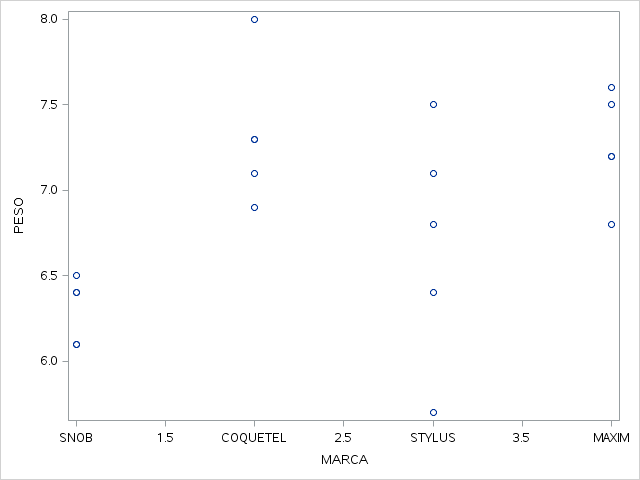
\includegraphics[scale=0.8]{scatterplot1}
    \caption{Gráfico de Dispersão para os Dados Experimentais vs Tratamento}
    \label{grafico:sp}
\end{figure}

\section{Análise e Intepretação}
\subsection{Análise de Variância}
    O Teste F para a inexistência do efeito do tratamento é ilustrado na Tabela \ref{tabela:anova} a seguir.

\begin{table}[htb]\label{tabela:anova}
\centering
    \begin{tabular}{c||p{17mm}|p{17mm}|p{17mm}|p{17mm}|p{17mm}}
         Fonte&g.l.&Soma de Quadrados&Quadrado Médio&Valor F&Pr $>$ F  \\\hline\hline
         Modelo& 3 & 3,5295&1,1765&6,03&0,0060 \\
         Erro& 16 & 3,12 &0,195\\\cline{1-3}
         Total Corrigido & 19 & 6,6495\\
    \end{tabular}
    \caption{Análise de Variância para os Dados Experimentais}
\end{table}

    Portanto a hipótese nula $H_0: \mu_1 = \mu_2 = \mu_3 = \mu_4$ pode ser rejeitada para estes dados e sob as suposições deste modelo (ver Estatísticas de Diagnóstico em \ref{sec:diagnostico}) com um nível alto de significância, já que temos um p-valor $<10^{-2}$ para $F = 6,03$. 
    
    Estabelecida a significância estatística da diferença entre as médias dos tratamentos, o interesse se volta para investigar com mais especificidade de que maneira estas diferenças se apresentam nos dados. Esa investigação posterior foi feita utilizando-se duas técnicas: contrastes ortogonais em \ref{sec:co} e comparações múltiplas utilizando o Teste de Dunnett em \ref{sec:cm}.
    
\subsection{Contrastes Ortogonais}\label{sec:co}

A Tabela \ref{tabela:estatisticas} a seguir apresenta Estatísticas úteis sobre as Medidas Experimentais: as médias dos tratamentos e geral, bem como os respectivos desvios padrões.

\begin{table}[htb]\label{tabela:estatisticas}
    \centering
    \begin{tabular}{c||c|c|c|c}
        Marca & 1 & 2 & 3 & 4   \\\hline
        Estatística & Snob & Coquetel & Stylus & Maxim \\\hline
        $\bar{y_{i.}}$&6,30&7,32&6,70&7,26\\
        $s_i$&$0,1870829$&$0,4147288$&$0,6892024$&$0,3130495$\\
        $n_i$&5&5&5&5\\
    \end{tabular}\caption{Estatísticas das Medidas Experimentais}
\end{table}

Em seguida, os 3 contrastes ortogonais\footnote{Como temos 4 tratamentos, o número máximo de contrastes ortogonais possíveis é 3} que foram estabelecidos antes do início do experimento são:

\begin{itemize}
    \item $l_1$: comparação entre os dois papeis-toalha de maior custo (Snob e Maxim) em relação aos dois de menor custo;
    \item $l_2$: comparação entre o papel-toalha mais caro (Snob) e o segundo mais caro (Maxim);
    \item $l_3$: comparação entre dois papeis fabricados pela mesma empresa\footnote{ver Anexo B em \ref{anexo:B}} e de custos semelhantes: Coquetel e Stylus.
\end{itemize}

Os coeficientes dos constrastes ortogonais são apresentados na Tabela \ref{tabela:coef_contrastes}, suas estimativas a partir dos dados experimentais estão na Tabela \ref{tabela:est_contrastes}, e o resumo do Teste F na Tabela \ref{tabela:teste_contrastes}






\begin{table}[htb]
    \centering
    \begin{tabular}{p{15mm} m{15mm} m{15mm} m{15mm} m{15mm} m{15mm} m{15mm} m{15mm}}
        ~&~&~Tratamento& \\\cline{2-5}
        ~& 1  &2 &3  &4 \\\hline
        Contraste & $a_1$&$a_2$&$a_3$&$a_4$&$\sum a_i^2$&$\hat{l}$&$SSC_i$\\\hline
        $l_1$&1/2&$-1/2$&$-1/2$&$1/2$&$1$&$-0,23$&0,2645\\\hline
        $l_2$&1&$0$&$0$&-1&2&$-0,96$&2,304\\\hline
        $l_3$&$0$&1&-1&0&2&$0,62$&0,961\\\hline
        $\hat{y}_{i.}$&6,30&7,32&6,70&7,26\\
    \end{tabular}
    \caption{Coeficientes utilizados nos Contrastes Ortogonais}
\label{tabela:coef_contrastes}
\end{table}

\begin{table}[htb]
    \centering
    \begin{tabular}{c||p{17mm}|p{17mm}|p{17mm}|p{17mm}|p{17mm}}
         Contrastes& Estimação&Erro padrão&IC inferior&IC superior  \\\hline\hline
        $\hat{l}_1$&$-0,23$ & 0,197&$-0,65$&0,19 \\
        $\hat{l}_2$&$-0,96$&0,279&$-1,55$&$-0,36$\\
        $\hat{l}_3$&0,62&0,279&0,03&1,21\\
    \end{tabular}\caption{Estimativas para os Contrastes Ortogonais}\label{tabela:est_contrastes}
\end{table}



\begin{table}[htb]
\centering
    \begin{tabular}{c||p{17mm}|p{17mm}|p{17mm}|p{17mm}|p{17mm}}
         Contrastes&g.l.&Soma de Quadrados&Quadrado Médio&Valor F&Pr $>$ F  \\\hline\hline
         1 e 4 vs. 2 e 3& 1 & 0,2645&0,2645&1,36&0,10 \\
         1 vs.4& 1 & 2,304&2,304&11,82&0,01\\
         2 vs.3& 1&0,961&0,961&4,93&0,01\\
    \end{tabular}\caption{Estatísticas do Teste F para os Constrastes Ortogonais}\label{tabela:teste_contrastes}
\end{table}

Considerando $\alpha_E = 0,05$ como o nível de significância para o experimento, utilizamos $\alpha_C = 1 - (1-\alpha_E)^{1/3} = 0,016$ como Limite Superior de tamanho $alpha_E$ para a probabilidade de cometer um Erro Experimental do Tipo I. Portando, a Tabela \ref{tabela:teste_contrastes} conclui o seguinte:

\begin{itemize}
    \item Para o \textbf{Contraste 1}: Não podemos rejeitar a hipótese de igualdade de médias de tratamento entre os dois papeis mais caros e os dois mais baratos, ou seja, eles absorvem em media a mesma quantidade de detergente quando considerados dois-a-dois;
    \item Para o \textbf{Contraste 2}: O papel-toalha mais caro (Tratamento 1 - Snob) apresenta absorção média de detergente \textbf{inferior} à da segunda marca mais cara (Tratamento 4 - Maxim), em média $0,96mL/10cm^2$ inferior;
    \item Para o \textbf{Contraste 3}: O papel-toalha da marca Coquetel é mais eficiente em absorver detergente em relação ao da marca Stylus, mesmo ambos sendo fabricados pela mesma empresa. Coquetel absorveu em média $0,62 mL/10cm^2$ de detergente a mais que Stylus.
\end{itemize}

%obs:Fiz os calculos considerando alpha =0,05, e não utilizei nenhum programa.por isso na tabela anova dos contrastes o p valor está exato (utilizei as tabelas do livro)

%comentario: 
%contraste 1: Os papéis toalha de maior custo absorveram em média a mesma quantidade de detergente que os papéis de custo inferior.(o contraste não é significativo); contraste2:O papel da marca Snob(mais cara) absorve em média 0,96ml/10cm2 a menos que a marca Maxim.(segunda mais cara); contraste 3: O papel da marca Coquetel absorveu em média 0,62ml/10cm2 de detergente a mais que o papel da marca Stylus sendo que ambos são da mesma fábrica e os de menor custo.

\section{Comparação com o melhor}\label{sec:cm}
O procedimento de comparações múltiplas com a melhor média das 
observações permite calcular o interesse da melhor observação em relação às demais. O Procedimento adotado foi o Método de Hsu.

No estudo em questão, a melhor observação refere-se à  marca de papel-toalha que obteve a maior média dos níveis de absorção de detergente: Tratamento 2 - Coquetel. Os parâmetros de interesse são $\mu_i - \max_{j\neq i} \mu_j$, com $i = \bar{1,4}$. O primeiro passo é calcular as diferenças entre cada tratamento em relação ao melhor deles, o Tratamento 2. A Tabela \ref{tabela:diferencas} a seguir apresenta este resultado

\begin{table}
\centering
    \begin{tabular}{c|c|c|c|c}
         Tratamento & 1 & 2 & 3 & 4  \\\hline
         $D_i$&$-1,02$&$0$&$-0,62$&$-0,06$ 
    \end{tabular}
    \caption{Diferenças entre os tratamentos e o melhor}\label{tabela:diferencas}
\end{table}

O passo seguinte é obter uma estimativa para a constante M, dada por $M = d_{\alpha,k,\nu}\sqrt{\frac{2s^2}{r}}$. Usando $\alpha = \alpha_E = 0,05$. $k = t-1 = 3$ e $\nu = gl(MSE) = 16$, $s^2 = MSE = 0,195$, temos $M = 0,7233$. A Tabela \ref{tabela:hsu} a seguir ilustra as estatísticas do Método em questão.

\begin{table}[!htb]
    \centering
    \begin{tabular}{{p{20mm}|c|c|c|c|c|c}}
         Tratamento& $\bar{y}_i$ & $\max_{j\neq i} \mu_j$ & $D_i$ & $D_i - M$ & $D_i + M$ & $(L;U)$ \\\hline
         1 & 6,3&7,32&$-1,02$&$-1,7433$&$-0,2967$&$(-1,7433;0)$\\
         3 & 6,7&7,32&$-0,62$&$-1,3433$&$0,1033$&$(-1,3433;0,1033)$\\
         4 & 7,26&7,32&$-0,06$&$-0,7833$&$0,6633$&$(-0,7833;0,6633)$\\
    \end{tabular}
    \caption{Estatísticas do Método de HSU para a Comparação entre o melhor (Tratamento 2) com os outros}
    \label{tabela:hsu}
\end{table}

Um intervalo com limite inferior igual a zero, indica que ele é o melhor tratamento.O tratamento 1 possui limite superior igual a zero e, portanto, não é o melhor. Em relação aos tratamentos 3 e 4 não fica claro qual o melhor,  uma vez que ambos os intervalos incluem zero, com nível de confiança de 95%.



\section{Diagnóstico}\label{sec:diagnostico}

\subsection{Análise Gráfica}
Para sustentar a validade do Modelo de Médias escolhido, foi verificada a adequabilidade dos dados experimentais em relação às suposições do Modelo. De particular interesse é a suposição de \textit{homocedasticidade}, isto é, de variância constante para as observações. A análise é resumida nos gráficos a seguir:

\begin{figure}[!htb]
    \centering
    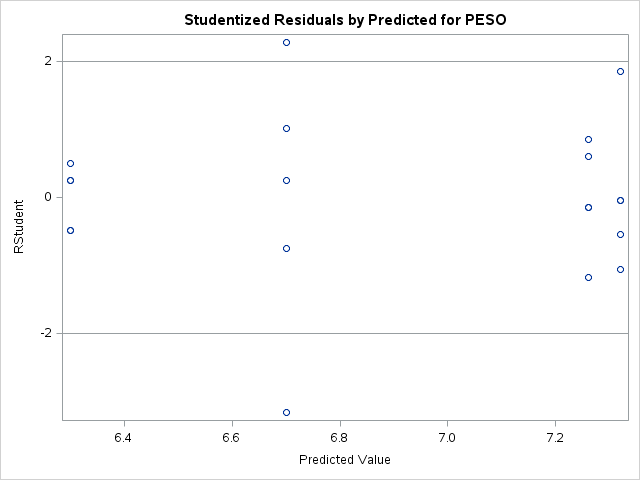
\includegraphics[scale=0.8]{res_student}
    \caption{Resíduos Studentizados Preditos para o Modelo}
    \label{grafico:res_student}
\end{figure}

\begin{figure}[!htb]
    \centering
    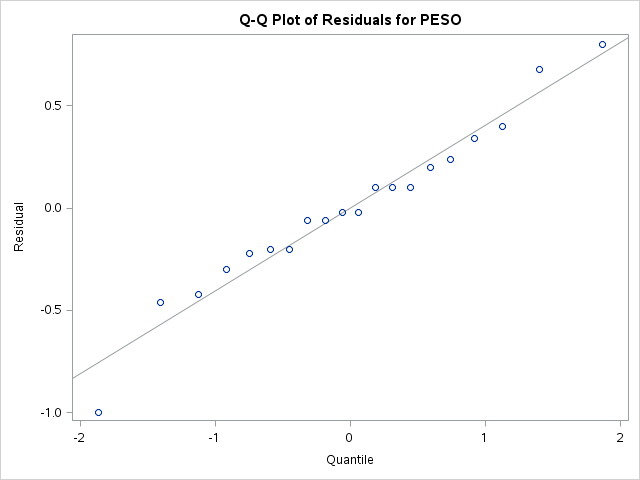
\includegraphics[scale=0.8]{qq-residuos}
    \caption{Gráfico de Probabilidade Normal para os Resíduos}
    \label{grafico:res_qqplot}
\end{figure}

\begin{figure}[!htb]
    \centering
    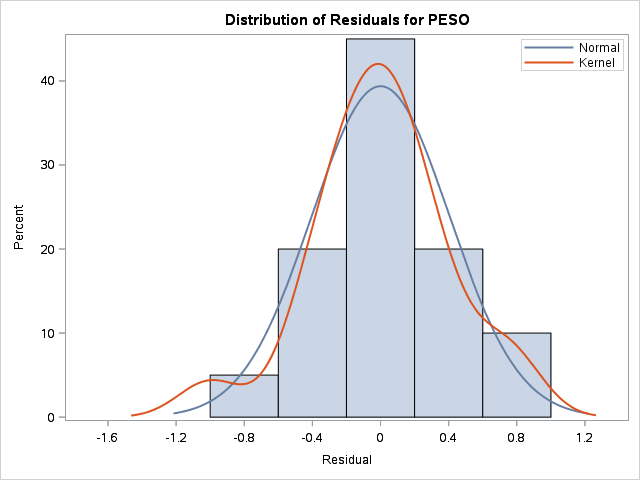
\includegraphics[scale=0.8]{dist_residuos}
    \caption{Distribuição dos Resíduos}
    \label{grafico:dist_residuos}
\end{figure}

    A análise gráfica serve mais como inspeção do que como verificação formal das suposições do modelo, de qualquer maneira, pelos gráficos podemos comentar o seguinte:
    
    \begin{itemize}
        \item O Gráfico \ref{grafico:res_student} mostra uma \textit{aparente} uniformidade dos resíduos, com exceção de dois \textit{outliers} que se encontram a mais de dois desvios padrões de suas respectivas distribuições amostrais;
        \item O Gráfico \ref{grafico:res_qqplot} de Probabilidade Normal mostra um ajuste \textit{de certa forma} decente dos resíduos com relação à distribuição de quantis da Distribuição Normal, e portanto \textit{sugere} que os resíduos têm sim Distribuição Normal;
        \item O Gráfico \ref{grafico:dist_residuos} é mais uma sugestão de que a hipótese de Normalidade não foi violada, é perceptível o quanto a distribuição dos resíduos é \textit{próxima} da Normal
    \end{itemize}
    \newpage
\subsection{Teste de Levene}
    O Teste de Levene é um teste não-robusto\footnote{Sensível à média} que avalia a igualdade de variâncias entre grupos como hipótese nula. Poderia ter sido escolhido outro Teste, não-paramétrico\footnote{Como o de Brown-Forsythe}, já que temos 2 \textit{outliers} nos nossos dados, mas como vimos no Gráfico \ref{grafico:dist_residuos}, a presença deles não introduz uma assimetria tão grosseira a ponto de invalidar o Teste. A Tabela \ref{tabela:levene} a seguir ilustra os resultados do Teste de Levene.
    
    \begin{table}[!htb]
        \centering
        \begin{tabular}{c||p{17mm}|p{17mm}|p{17mm}|p{17mm}|p{17mm}}
         Fonte&g.l.&Soma de Quadrados&Quadrado Médio&Valor F&Pr $>$ F  \\\hline\hline
             Marca & 3 & 0,3646 & 0,1215 & 2,15 &  0,1344\\
             Erro & 16 &0,9058 & 0,0566
        \end{tabular}
        \caption{ANOVA da Soma dos Desvios Quadráticos das Médias dos Grupos}
        \label{tabela:levene}
    \end{table}
    
    Como a hipótese nula é de que os grupos têm mesma variância, deixamos de rejeitá-la com uma significância $>0,13$, validando assim a suposição de homocedasticidade.
    
    
\subsection{Teste de Aleatoriedade de Wald-Wolfowitz}
    O teste em questão avalia uma hipótese nula de aleatoriedade, em particular para os resíduos do Modelo em questão. Para os dados experimentais, obtemos $p \approx 1$, o que não-rejeita a hipótese de aleatoriedade dos resíduos.

\section{Poder do Teste e Tamanho de Amostra para Experimentos Futuros}
    O cálculo do Poder do Teste é essencial para qualquer procedimento estatístico, seja ele observacional ou experimental. O Poder do Teste aumenta com o tamanho da amostra ou do número de repetições experimentais, mas a um custo que pode ser não-negligenciável. No caso deste experimento, o custo financeiro é irrisório, mas em termos de tempo o trabalho mostrou-se dispendioso. 
    
    Já para o tamanho da amostra necessário do Teste temos um raciocínio em certo sentido inverso: qual o tamanho da amostra para atingir tal Poder do Teste? Essa medida é de grande utilidade na ciência, pois pode servir como ponto de partida para investigações posteriores, mais refinadas. 
    
    Utilizamos então as estimativas encontradas neste experimento para a variância $\sigma_e$, e seguimos então ao cálculo do teste para a hipótese nula do Modelo de Médias, a igualdade entre as médias dos tratamentos, e obtivemos o 0,898 como poder para o teste de médias. Esse poder parece ser alto o suficiente para os propósitos práticos do experimento, um bom equilíbrio entre número de observações e poder. Se quiséssemos um poder de 0,98, por exemplo, teríamos de ter 40 observações no total, 10 em cada grupo. O dobro do trabalho para um aumento de $\approx 8\%$ no poder.

\section{Conclusão}

Como pode se observar, há sim diferenças entre as marcas para a absorção do detergente. O Modelo de Médias escolhido retratou esse fato implicando numa diferença nas Médias de Tratamento. Chama-se atenção a um resultado curioso: a relação entre preço e a capacidade de absorção não seguiu como se previa. A marca mais cara (Snob), não obteve uma capacidade de absorção maior que as demais, cedendo esse posto à marca Maxim. Graças aos Contrastes Ortogonais e a Comparação com o Melhor verificou que o papel-toalha mais dispendioso pode não ser o melhor. Desse modo, devido a essas técnicas de delineamento experimental, a relação custo benefício da marca Maxim é possivelmente maior. Por outro lado, essa relação cai na marca Snob, não compreendendo-se por ela ser tão cara.
\bibliographystyle{abbrv}
\nocite{kuehl1994statistical}
\nocite{kuehl2001diseno}
\nocite{kutner2003applied}
\nocite{lawson2010design}
\bibliography{Experimento1-DAE-Grupo1}
\newpage

\section{Anexo A - Códigos}\label{anexo:A}

    Todos os códigos deste Trabalho, inclusive microdados e relatório em .tex, estão disponível em um repositório no serviço github: \url{https://github.com/august-o/Experimento1-DAE}

\subsection{Códigos em R}
\begin{lstlisting}[language=R]

# Escolha das amostras dos papeis
sample.int(120,5,replace=FALSE)
# [1] 12 59 43 50 35
set.seed(30)
sample.int(60,5,replace=FALSE)
#[1]  6 29 22 24 17
set.seed(30)
sample.int(50,5,replace=FALSE)
#[1]  5 24 18 20 14
set.seed(13)
sample.int(60,5,replace=FALSE)
#[1] 43 15 23  6 54


# Dados
marcas <- factor(rep(
c("Snob", "Coquetel", "Stylus", "Maxim"), each = 5))
delta.peso <- c(6.4,6.4,6.1,6.1,6.5,6.9,
7.3,8,7.3,7.1,5.7,6.4,7.1,6.8,7.5,7.5,6.8,7.2,7.6,7.2)
dados <- data.frame(peso = delta.peso, marcas)

attach(dados)


#Media e dp para os tratamentos
tapply(peso,marcas,mean)
tapply(peso,marcas,sd)

#Anova e Predicao
anova.papeis <- aov(peso~marcas)
summary(anova.papeis)
predict(anova.papeis)

#Teste de Wald-Wolfowitz para Aleatoriedade
require("randtests")

runs.test(residuals(anova.papeis), plot = T)
\end{lstlisting}

\subsection{Códigos em SAS}
\begin{lstlisting}[language=SAS]
PROC FORMAT;
	VALUE MARCA 1 = 'SNOB'
			2 = 'COQUETEL'
			3 = 'STYLUS'
			4 = 'MAXIM';
			RUN;
	
DATA EXPERIMENTO1;
	FORMAT MARCA MARCA.;
	INPUT MARCA PESO @@;
	DATALINES;
1 6.4 1 6.4 1 6.1 1 6.1 1 6.5
2 6.9 2 7.3 2 8.0 2 7.3 2 7.1
3 5.7 3 6.4 3 7.1 3 6.8 3 7.5
4 7.5 4 6.8 4 7.2 4 7.6 4 7.2
;

PROC SGPLOT DATA = EXPERIMENTO1;
	SCATTER Y=PESO X= MARCA;
	RUN;
	
PROC GLM DATA = EXPERIMENTO1 PLOTS=DIAGNOSTICS(UNPACK);
CLASS MARCA;
MODEL PESO = MARCA/SOLUTION;
RUN;
PROC GLM DATA=EXPERIMENTO1 PLOTS=DIAGNOSTICS;
  CLASS MARCA;  
  MODEL PESO=MARCA;
  MEANS MARCA / HOVTEST=LEVENE;
  OUTPUT OUT=RESI R=R;
RUN;
QUIT;

PROC UNIVARIATE DATA=RESI NORMAL PLOT;
VAR = R;
RUN;

PROC RANK DATA=EXPERIMENTO1 OUT=REXPERIMENTO1;
  VAR PESO;
RUN;

PROC GLM DATA=REXPERIMENTO1;
  CLASS MARCA;
  MODEL PESO=MARCA;
RUN;

TITLE3 'KRUSKAL-WALLIS - UTILIZANDO NPAR1WAY';

PROC NPAR1WAY DATA = EXPERIMENTO1;
  CLASS MARCA;
  VAR PESO;
RUN;

PROC GLMPOWER DATA=EXPERIMENTO1;
	CLASS MARCA;
	MODEL PESO = MARCA;
	POWER
  		STDDEV = 0.441588
    	ALPHA  = 0.05
   		NTOTAL = 20
    	POWER  = . ;
RUN; 


PROC GLMPOWER DATA=EXPERIMENTO1;
	CLASS MARCA;
	MODEL PESO = MARCA;
	POWER
  		STDDEV = 0.441588
    	ALPHA  = 0.05
   		NTOTAL = .
    	POWER  = 0.98 ;
RUN;
\end{lstlisting}

\newpage
\section{Anexo B - Fotos dos Procedimentos}\label{anexo:B}
As fotos a seguir ilustram alguns estágios do procedimento experimental descrito em \ref{sec:procedimentos}.

\begin{figure}[!htb]
    \centering
    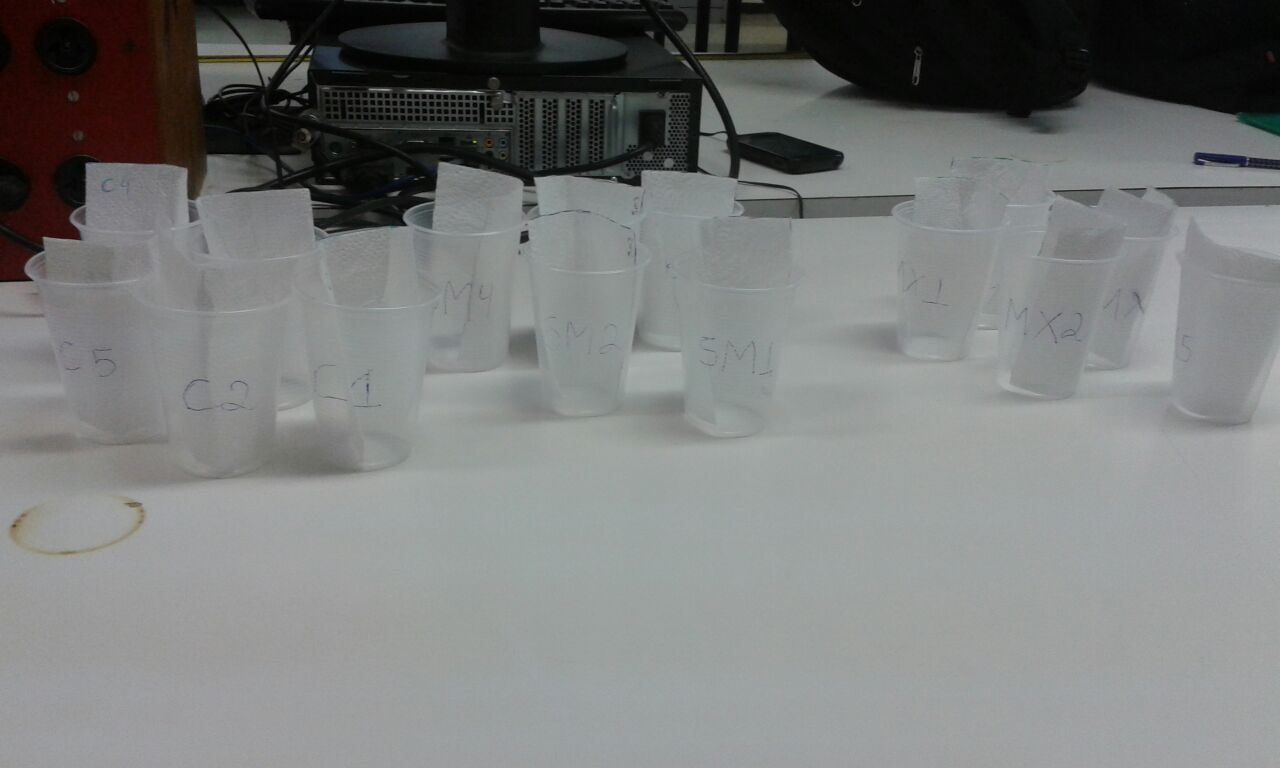
\includegraphics[scale = 0.27]{foto1}
    \caption{Quadrados de 10cm x 10cm dentro dos copos, rotulados por marca e observação}
    \label{fig:foto1}
\end{figure}

\begin{figure}
    \centering
    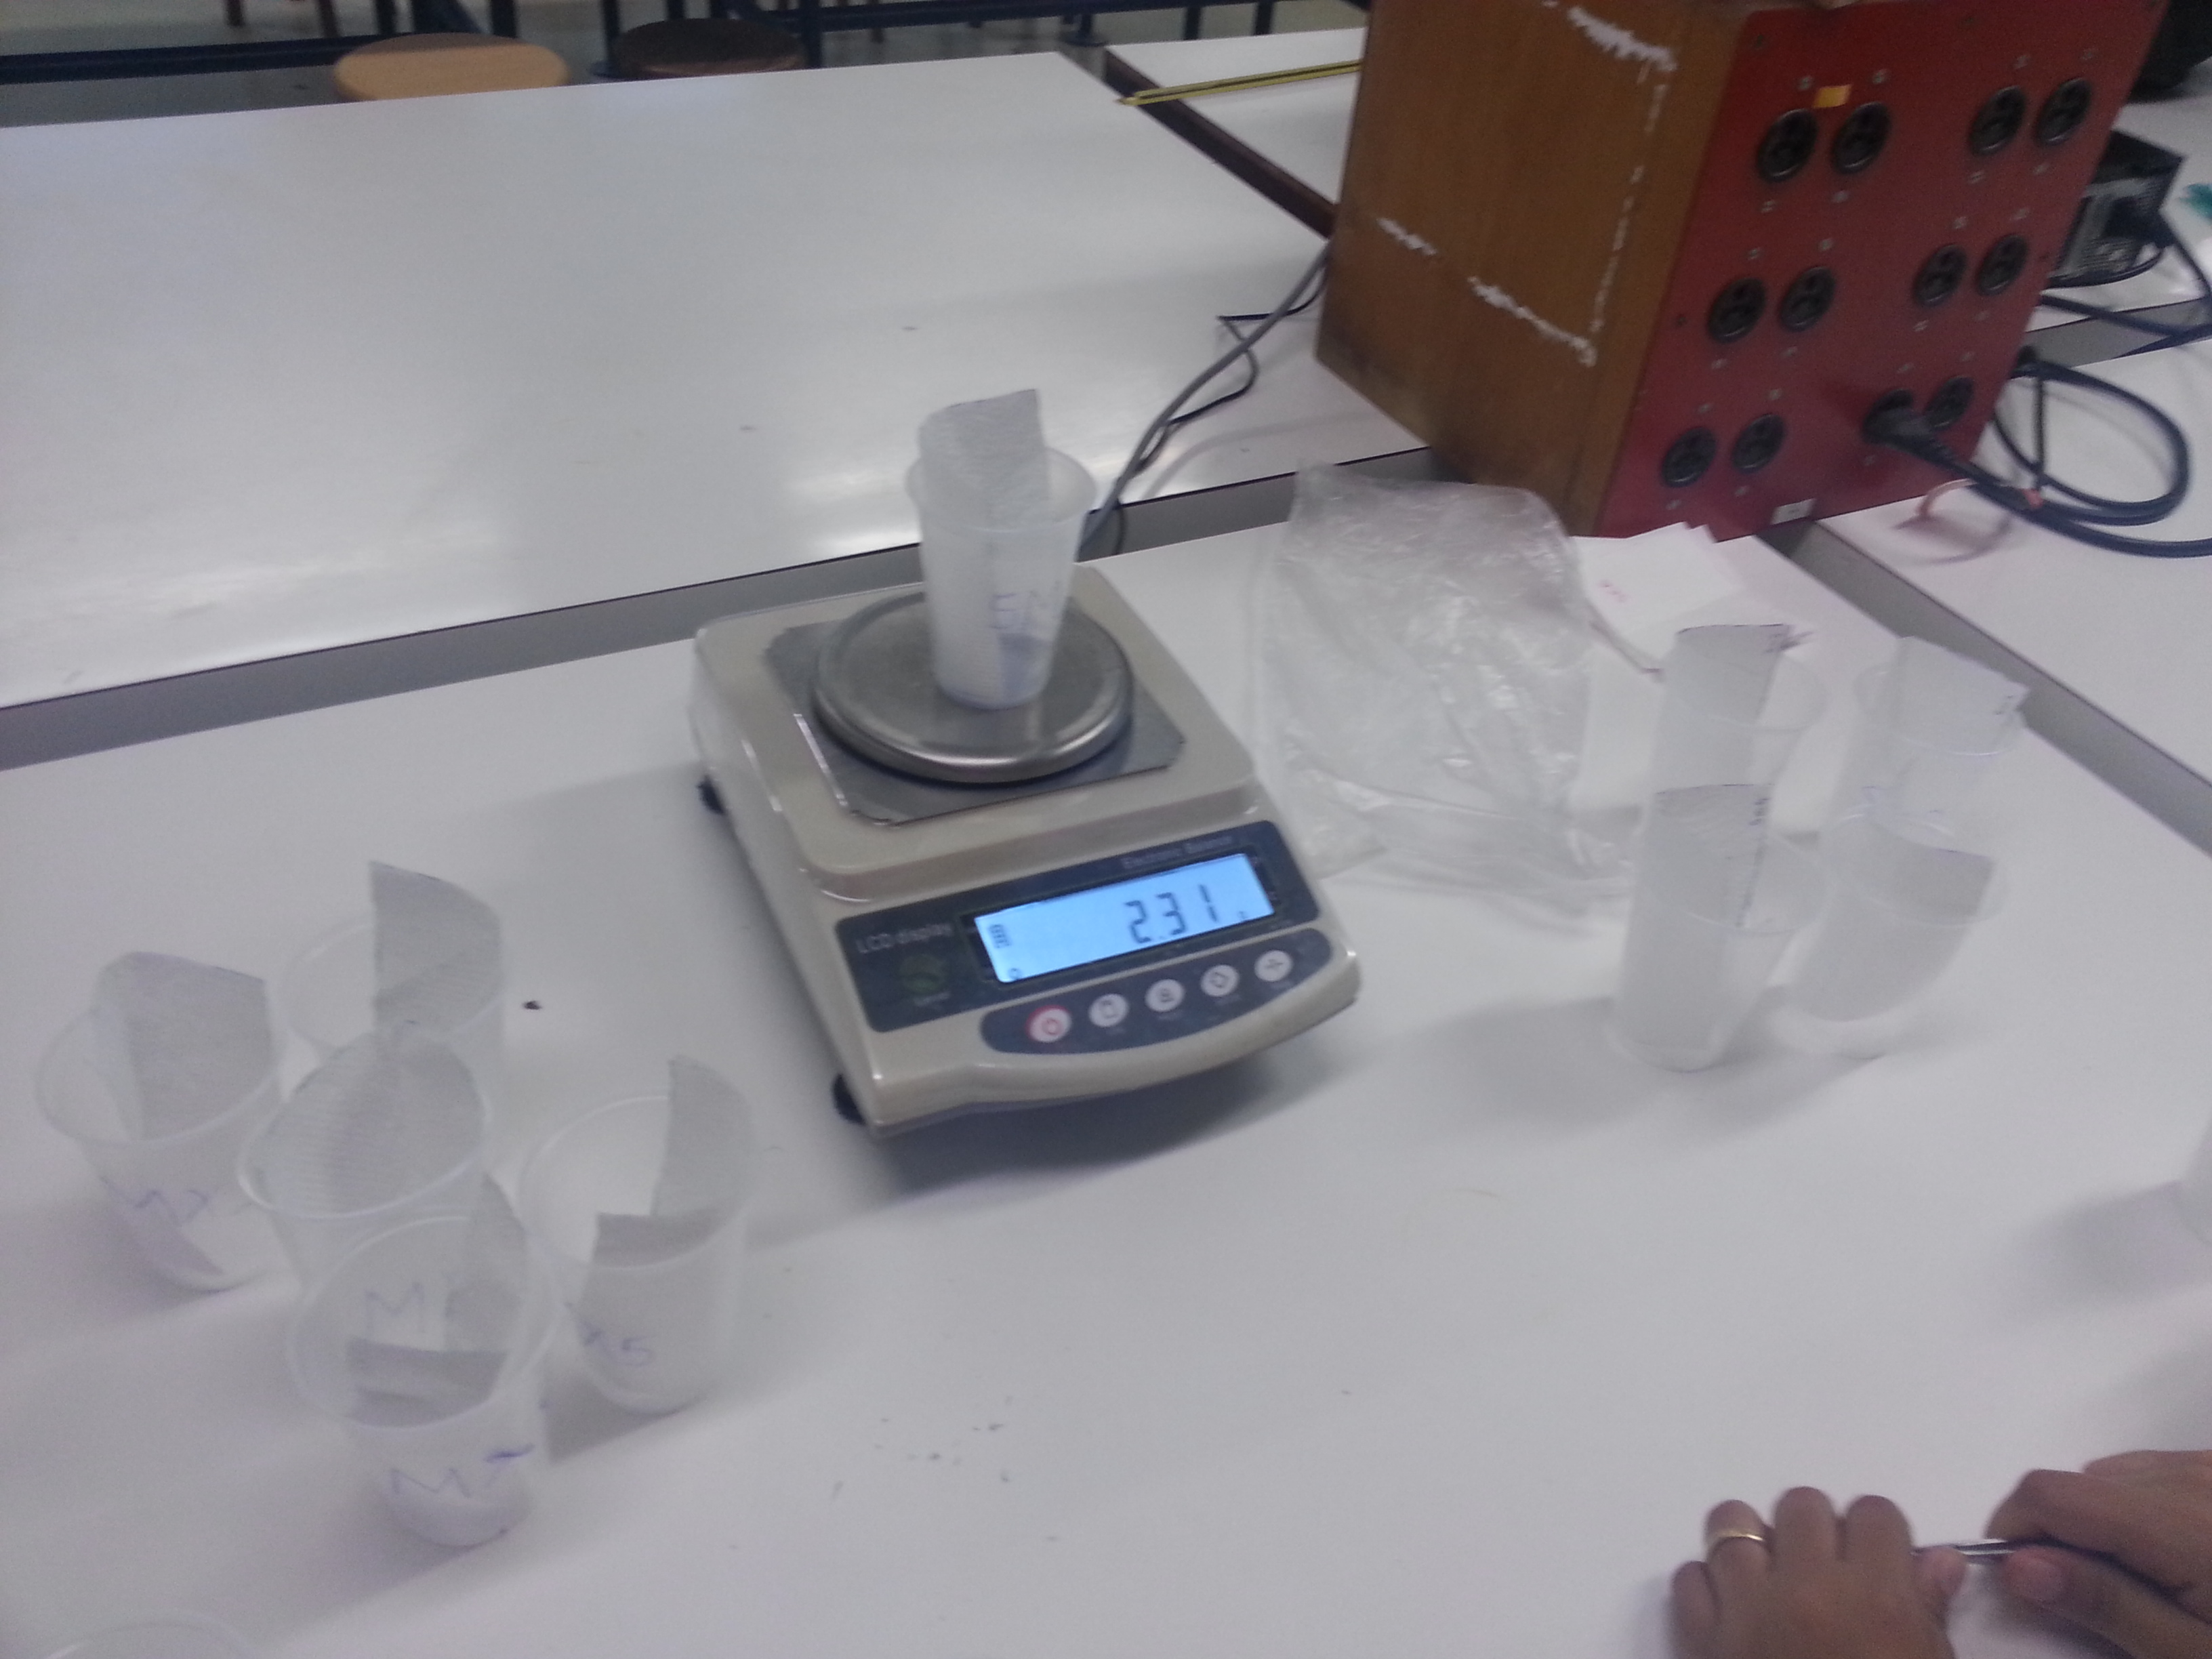
\includegraphics[scale=0.11]{foto2}
    \caption{Mensuração do \textit{Peso Seco}}
    \label{fig:foto2}
\end{figure}

\begin{figure}
    \centering
    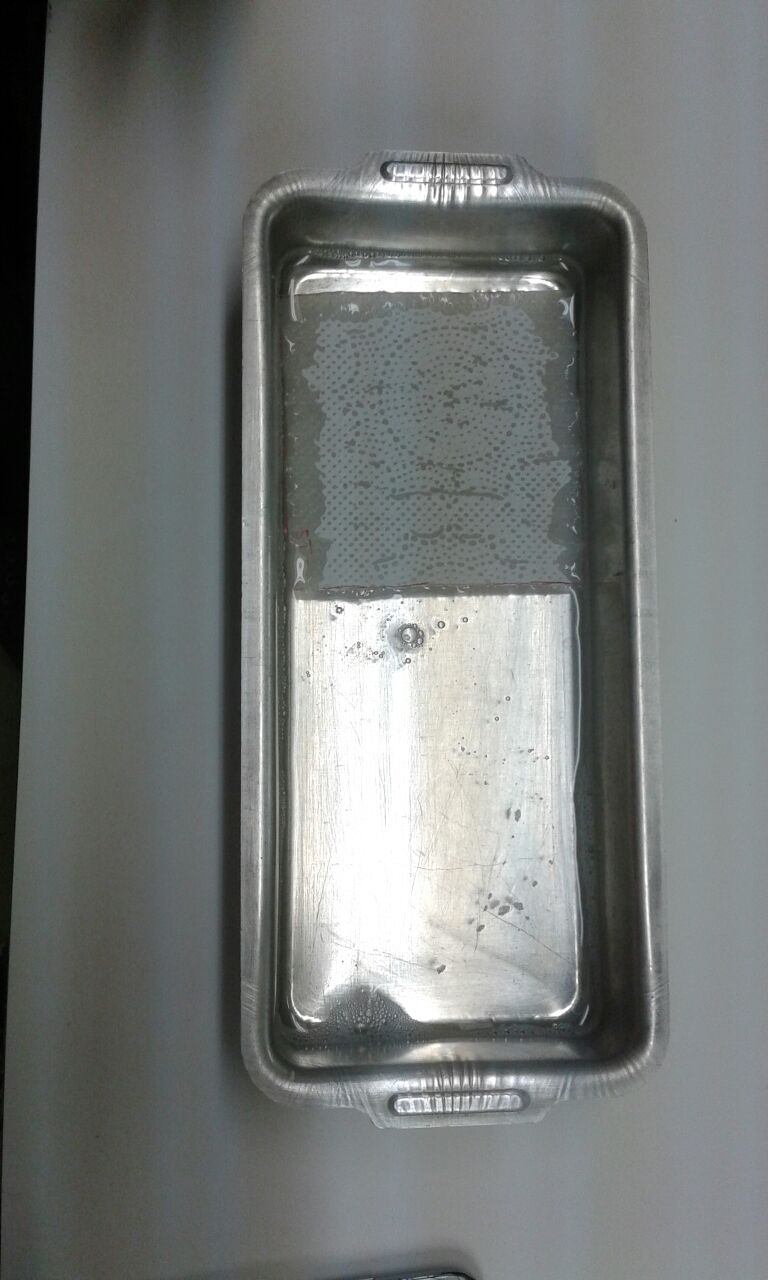
\includegraphics[scale = 0.3]{foto3}
    \caption{Folha de papel-toalha repousando sobre o detergente dentro da forma de alumínio}
    \label{fig:foto3}
\end{figure}

\begin{figure}
    \centering
    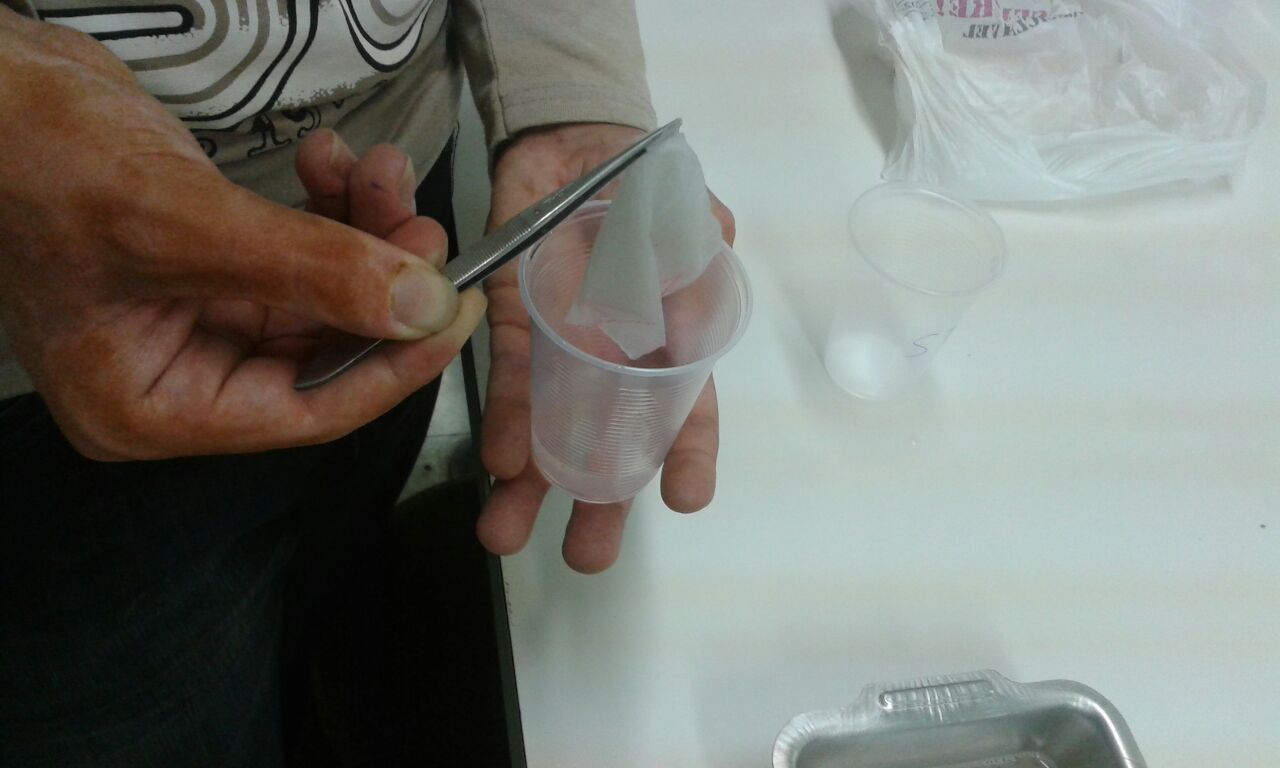
\includegraphics[width=\textwidth]{foto4}
    \caption{Escorrimento do excesso de detergente no papel durante 60 segundos}
    \label{fig:foto4}
\end{figure}

\begin{figure}
    \centering
    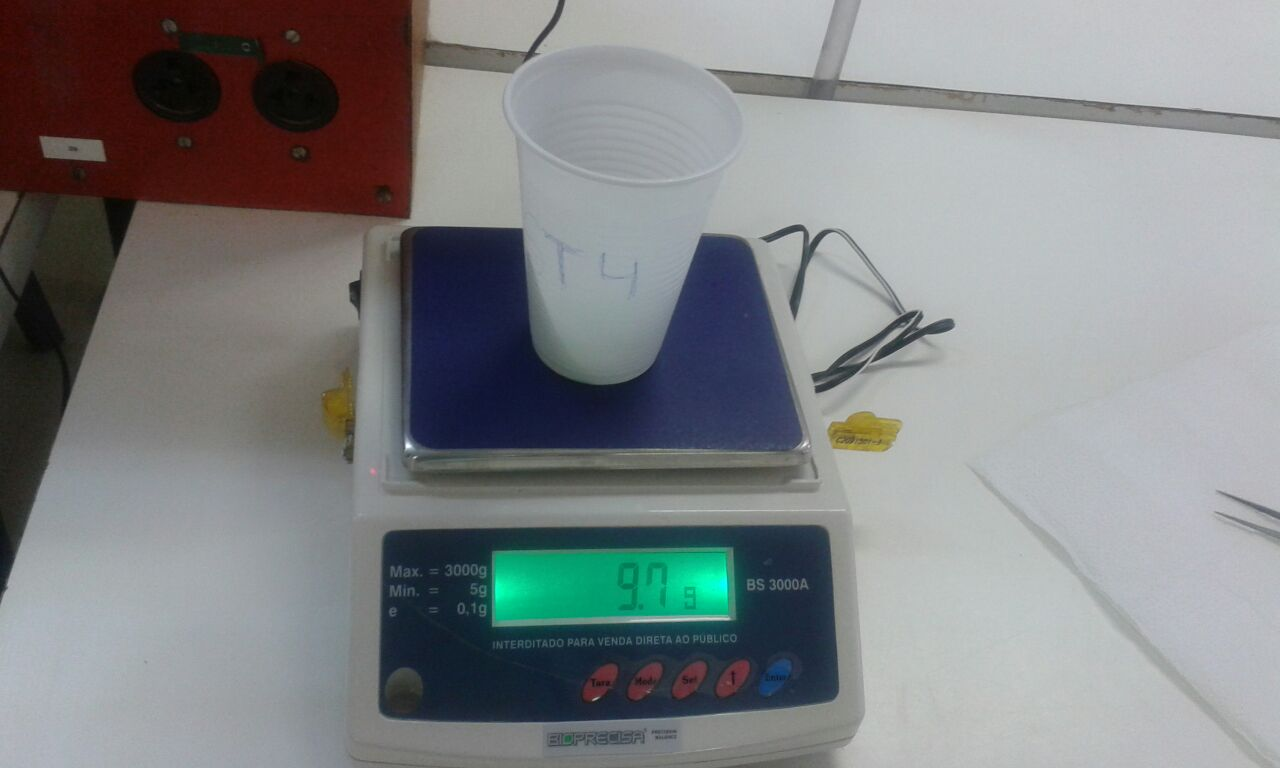
\includegraphics[width=\textwidth]{foto5}
    \caption{Mensuração do \textit{Peso Úmido}}
    \label{fig:foto5}
\end{figure}


\end{document}
